
%%%%%%%%% Sample inclusion of a figure
 % \begin{figure}[h]
 % \begin{center}
 % 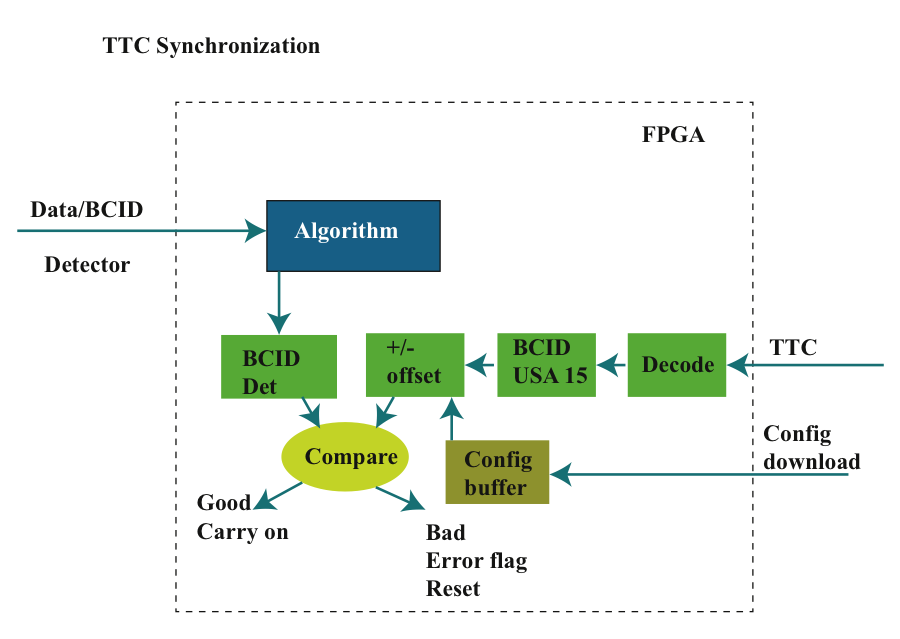
\includegraphics[width=0.8\textwidth]{specs/Diagram-TTCSync}
 % \caption{Block diagram of an implementation of the TTC synchronization.}
 % \label{fig:Monitoring}
 % \end{center}
 % \end{figure}


The ART (address in real time) data from an entire sector will be transmitted to a single
trigger processor via 32 ADDCs. Each ADDC will transmit its data on a
single fiber optic link. The trigger processor therefore uses 32
fibers to receive the ART data from one sector. The
MM and sTGC trigger processors will share the same ATCA carrier card
and each carrier will support two sectors.

\subsubsection{ART Data Protocol}

The ART Data from the ADDC will be transmitted using the GigaBit Transceiver
(GBT) architecture and transmission protocol in a low-latency widebus
mode at a rate of 4.8 Gb/s. The trigger processor will take advantage of the GBT firmware
developed by the GBT Project to implement the receivers.

The GBT packet in widebus mode will provide 112 data bits and arrives
once every bunch crossing. One ADDC will service 32 VMMs and each
packet can contain ART data from a maximum of eight triggered VMMs. Each
VMM will be uniquely identified to determine which MM strip
on the sector is hit.

There are two options for how data packet bits is defined. The
difference between the two is how the VMM ID information is encoded.
The first data protocol option will provide the VMM IDs of every VMM
that was triggered by asserting a bit in a 32-bit hit list as shown in 
Figure~\ref{fig:addcGbtFormat2}. The second
option will encode each VMM ID in a list. For both options, the triggered
strip number within each VMM will be provided in an encoded list. The first
option would move the VMM ID encoding task from the ADDC ASIC to the
trigger processor FPGA. 
Both options, shown in Tables~\ref{tab:ARTfmt_opt1} and
~\ref{tab:ARTfmt_opt2}, use the full 112~bits provided by the GBTx' wide mode.

\begin{figure}[h]
  \begin{center}
    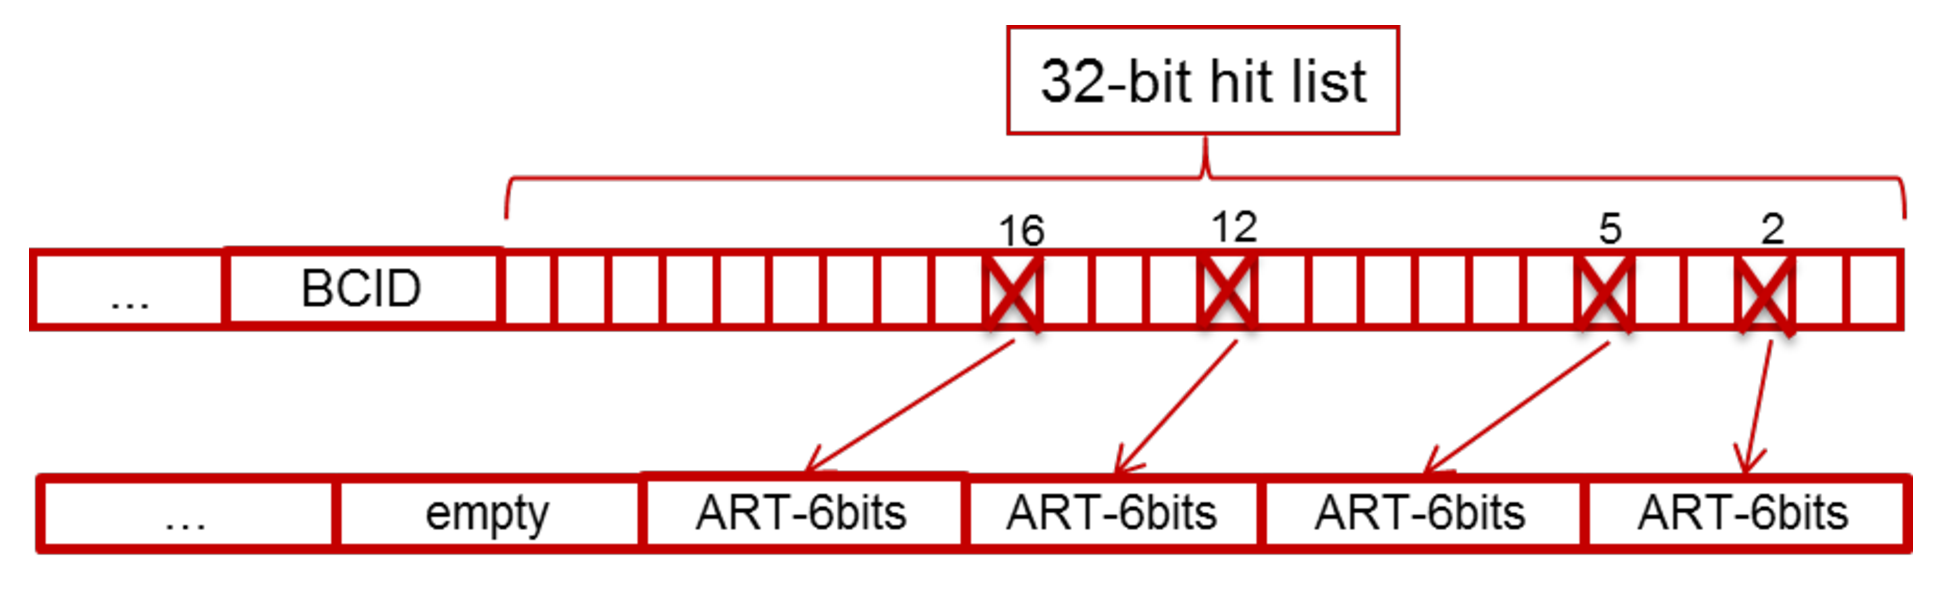
\includegraphics[width=0.6\textwidth]{figures/specs/addcGbtFormat2.pdf}
    \caption{Option 1 VMM ID encoding using 32-bit hit list.}
    \label{fig:addcGbtFormat2}
  \end{center}
\end{figure}


\begin{table}[htbp]
  \centering
    \begin{tabular}{|c|c|c|c|c|c|}
    \hline
    0b1010 & BCID(12) & ERR\_FLAGS(8) & HIT\_LIST(32) & ARTDATA\_PARITY(8) & 8xART\_DATA(6) \\
    \hline
    \end{tabular}\caption{Option 1 ADDC GBT packet format.}
  \label{tab:ARTfmt_opt1}%
\end{table}%

\begin{table}[htbp]
  \centering
    \begin{tabular}{|c|c|c|c|c|}
    \hline
    HIT\_CNT(3) & BCID(12) & 8xVMMID(5) & ARTDATA\_PARITY(8) & 8xART\_DATA(6) \\
    \hline
    \end{tabular}\caption{Option 2 ADDC GBT packet format.}
  \label{tab:ARTfmt_opt2}%
\end{table}%


\begin{comment}
{\small
\begin{tabular}{|c|c|c|c||c|c|}
\hline
\multicolumn{6}{|c|}{Option 1 GBT DATA{[}111:0{]}}\tabularnewline
\hline
\hline
``1010''  & BCID{[}11:0{]}  & ERR\_FLAGS{[}7:0{]}  & HIT\_LIST{[}31:0{]}  & ART\_PARITY{[}7:0{]}  & 8 x ARTDATA{[}5:0{]}\tabularnewline
\hline
\end{tabular}

\begin{tabular}{|c|c|c||c|c||c|}
\hline
\multicolumn{6}{|c|}{Option 2 GBT DATA{[}111:0{]}}\tabularnewline
\hline
\hline
HIT\_CNT{[}3:0{]}  & BCID{[}11:0{]}  & \multicolumn{2}{c|}{8 x VMMID{[}4:0{]}} & ART\_PARITY{[}7:0{]}  & 8 x ARTDATA{[}5:0{]}\tabularnewline
\hline
\end{tabular}
}  % end small

\end{comment}

%\begin{description}
%\item [BCID] = 12 bit bunch crossing ID 
%\item [HIT\_LIST] = 32-bit list of flags corresponding to each of
%the 32 VMMs. 0 - no hit, 1 - hit. A register controls if this is a
%filtered (i.e. 8 hits max) or an unfiltered copy of the VMM flags
%registered in a particular BC.
%\item [HIT\_CNT] = 4-bit  number of hits (range 0 - 8; 9 - 15 invalid)
%\item [VMMID] = 5-bit address of triggered VMM
%\item [ART\_DATA] = 6-bit triggered VMM strip number
%\item [ARTDATA\_PARITY] = 8-bit parity the ART data computed by
%each of the 32 ART de-serializer units. Each bit corresponds to one
%of the ART data field selected by the priority unit.
%\end{description}

\begin{itemize}
\item BCID = 12 bit bunch crossing ID 
\item HIT\_LIST = 32-bit list of flags corresponding to each of
the 32 VMMs. 0 - no hit, 1 - hit. A register controls if this is a
filtered (i.e. 8 hits max) or an unfiltered copy of the VMM flags
registered in a particular BC.
\item HIT\_CNT = 4-bit  number of hits (range 0 - 8; 9 - 15 invalid)
\item VMMID = 5-bit address of triggered VMM
\item ART\_DATA = 6-bit triggered VMM strip number
\item ARTDATA\_PARITY = 8-bit parity the ART data computed by
each of the 32 ART de-serializer units. Each bit corresponds to one
of the ART data field selected by the priority unit.
\end{itemize}


\subsubsection{Decoding ART Data}

Once the ADDC GBT packet is received, the ART data is decoded into a strip number.  This number represents the  strip's distance to the beam line.  Each fiber will have an associated  geographic address that is used in the decoding process to set the location of strip 0.  The strip number is then multiplied by a constant to calculate the slope of a line with the interaction point.  The slopes for each ART hit are then sent, along with the strip number, to the trigger processor algorithm.
Since the fiber location will provide information used to calculate the strip number, the ADDC will have a debug mode that can be used to diagnose cabling issues.
